\documentclass[conference]{IEEEtran}

\usepackage{draftwatermark}
\usepackage[backend=bibtex]{biblatex}

\addbibresource{report.bib}
\nocite{*}

\begin{document}

	\title{Lag compensation techniques for networked games}
	\author{\IEEEauthorblockN{James Robinson}
	\IEEEauthorblockA{Electronics and Computer Science\\
	University of Southampton\\
	Email: jr4e09@soton.ac.uk}}
	\maketitle

	\begin{abstract}
		In networked multiplayer games, network latency often introduces an unacceptable delay between when the player attempts to take an action and when the action actually takes effect within the game world. In this paper, methods of quantifying the effects of this latency, algorithms that mask its apparent effects, and a selection of novel unified frameworks for lag compensation are explored. Also discussed are the advantages and limitations of each algorithm, along with their potential applications.
	\end{abstract}

	\section{Introduction}

	% Explain what kinds of games we're talking about and general terminology
	% Assume tick-based games

	In gaming, the term ``lag'' refers to the delay between when the user takes an action, and when the action takes effect within the game world. Lag can be introduced by many factors including input device latency, framerate, vsync, and monitor response time, but the most egregious source of lag in networked or online games is the latency between client and server. Although techniques exist to reduce this latency, the fact that data transfer is limited by the speed of light means that this latency can never be completely eliminated.

	Lag reduces player engagement and enjoyment, and furthermore can impact performance in competitive multiplayer games \cite{beigbeder2004effects}. For this reason, most popular online games take measures to reduce the effect of network latency on the player's experience. Such techniques are generally referred to as ``lag compensation'' algorithms. Many such techniques exist, each of which make various tradeoffs that are appropriate for some types of game. Because of the disparate requirements of different genres of game, no ``silver bullet'' solution exists.

	In this paper, I will introduce various state of the art techniques for lag compensation in networked multiplayer games, discussing their advantages and disadvantages, as well as which types of simulation each technique is suited to. I will also present some unified models.

	\section{Quantifying effects of latency}

	TODO \cite{beigbeder2004effects} \cite{chen2011perceptual} \cite{claypool2005effect} \cite{fritsch2005effect} \cite{sheldon2003effect} \cite{quax2004objective} \cite{dick2005analysis}

	\section{Dead reckoning}

	The simplest form of client-side lag compensation is ``dead reckoning'' (named for the principle used in navigation). Under this approach, the last known positions and velocities of each game object are used to predict their current position via extrapolation, taking latency into account. For example, given current time $t$, current latency $l$, and a game object with last known position $\hat{s}_{t - l}$ and velocity $\hat{v}_{t - l}$, the predicted position at the current point in time is $\hat{s}_{t} = \hat{s}_{t - l} + l\hat{v}_{t - l}$. Figure~\ref{fig:extrapolation_timeline} shows a timeline of this approach: updates from the server take some amount of time to reach the client, and the client extrapolates game object positions to predict where they are now.

	\begin{figure}
		\centering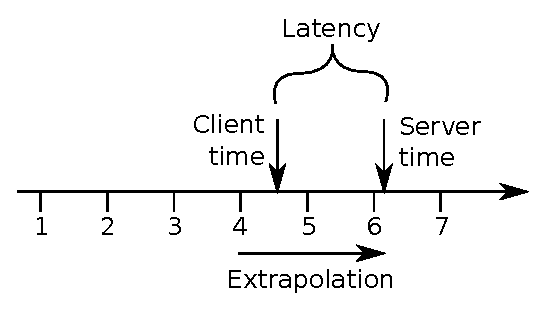
\includegraphics[width=\linewidth]{figures/extrapolation_timeline.eps}
		\caption{A timeline showing extrapolation. The client predicts the current server time based on measured latency, and extrapolates object positions from the position and velocity data in the latest update received from the server ($t = 4$).}
		\label{fig:extrapolation_timeline}
	\end{figure}

	Misprediction errors are very common under this scheme, occurring every time the velocity or bearing of a game object changes. The simplest way to correct misprediction errors is to immediately ``snap'' the object to the correct location once an update arrives from the server, but this can cause very visible visual discontinuities that can be distracting for the player. A less accurate but visually smoother approach is to interpolate between the position that the entity was last rendered at and its current estimated position (as shown in figure~\ref{fig:extrapolation}). This smooths out the visual discontinuities but also further reduces precision.

	\begin{figure}
		\centering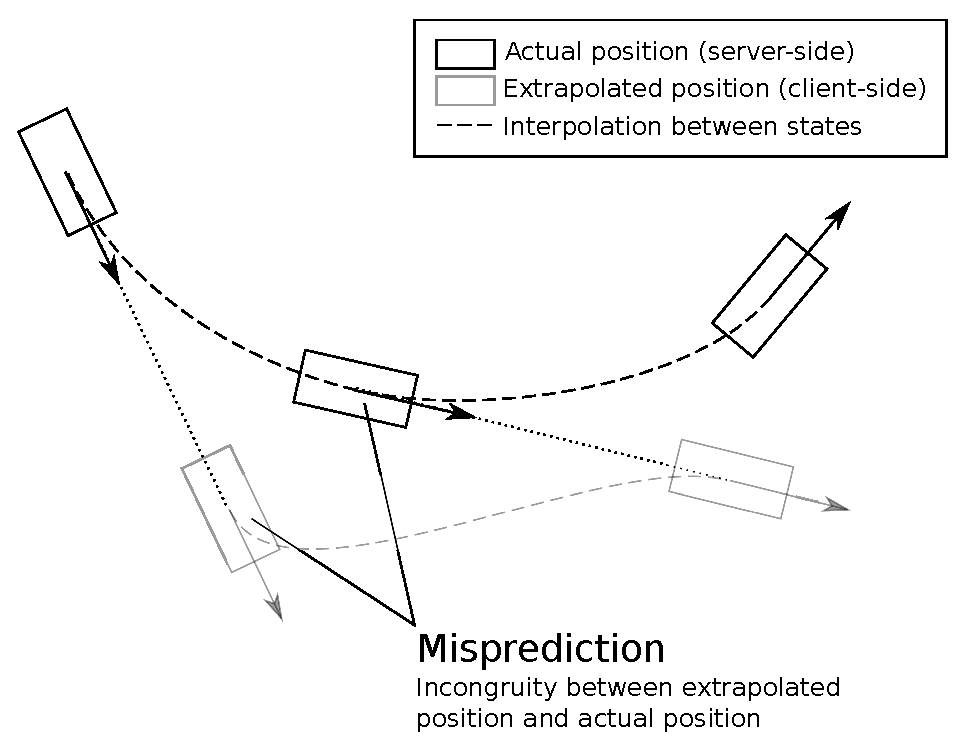
\includegraphics[width=\linewidth]{figures/extrapolation.eps}
		\caption{Misprediction. The client extrapolates object positions based on measured latency in order to predict where they are now. If objects change bearing, misprediction errors occur.}
		\label{fig:extrapolation}
	\end{figure}

	It is important to note that when using this scheme, game objects are very rarely (if ever) rendered at correct, accurate positions. This tradeoff is acceptable for some games, particularly where game objects change velocity or bearing reasonably slowly (for example, cars in a racing game) \cite{pantel2002suitability}, but for games requiring pinpoint accuracy, a better scheme is required.

	% Sometimes use high-order differential coefficients http://www.mine-control.com/zack/timesync/timesync.html

	\emph{On the Suitability of Dead Reckoning Schemes for Games}

	\begin{itemize}
		\item 2 different categories of prediction scheme: prediction of positions, and prediction of input events
		\item Position prediction
		\item Scheme 1: assume constant velocity and predict position from that
		\item Scheme 2: assume constant acceleration and predict velocity and hence position from that
		\item Scheme 3: same as scheme 2, but using Lagrange polynom with degree of 2 (commonly used for interpolation and extrapolation in 3D graphics)
		\item Scheme 4: Predict trajectory using constant velocity
		\item Input prediction
		\item Scheme 5: Predict position assuming constant control device (i.e. joystick) position
		\item Scheme 6: Predict position assuming constant control device velocity
		\item Scheme 7: Predict using Lagrange polynom and assuming constant control device acceleration
		\item Considered applications to 3 different game types: sports, 3D action (fps, tps), simulators/racing games
		\item For sports games, a cursor-like steering model was used
		\item For action games and racing games, the x axis controls direction and the y axis controls motion along that bearing
		\item Quality of prediction scheme is defined as difference between position calculated by game engine/server, and the predicted position, average deviation between actual and predicted taken
		\item Results were surprising: the most complex schemes did not always lead to the best results.
		\item Scheme 5 was very successful despite simplicity
		\item Scheme 6 worked best for sports games, with all input prediction schemes working well for this game type
		\item Scheme 7 worked best for action games
		\item Only position prediction schemes were evaluated for racing/simulation games because a proprietary physics engine was used, and scheme 2/3 performed best
		\item The paper claims that prediction drastically improved the experience for all game types, but fared worse for sports games because the characters move more eratically.
		\item Critical evaluation
		\item The model used to simulate action games in the paper is fairly unrealistic: characters in a first-person shooter do not behave like vehicles. Players can move freely in any direction rather than being constrained to motion in the direction they're facing, and tend to move very eraticalls
		\item Using input prediction schemes for a competitive multiplayer action game might be infeasible for the same reason that input prediction failed for racing/simulation games in the paper: most action games use proprietary physics engines and many of them involve incredibly complex interactions with the environment (destructible terrain, etc.) Prediction is very difficult in such games.
		\item Results are misleading at best: prediction probably doesn't work as well for action games as the authors claim, although they did present novel techniques for racing game prediction which perform better than the naive approach
	\end{itemize}

	\emph{http://www.mine-control.com/zack/timesync/timesync.html}

	\begin{itemize}
		\item NTP too complicated and takes a long time to converge, not ideal for games; the player expects to be able to jump straight in
		\item Paper also mentions that NTP relies on UDP which might be blocked by many ISPs including corporate WANs
		\item Proposes a very simple clock synchronisation algorithm built on TCP, essentially it's a moving average latency calculation
		\item Latency estimates are pushed into an ordered list periodically, and the median is taken
		\item Samples that are further away from the mean than 1 SD are assumed to be retransmissions, and are discarded
		\item Typically converges within about 100ms, which is plenty fast enough
		\item Implemented in NetStorm, Islands At War, a commercial RTS game, with good results
	\end{itemize}

	\emph{Accuracy in Dead-Reckoning Based Distributed Multi-Player Games}

	\begin{itemize}
		\item Focuses on accuracy
		\item Primarily applicable to distributed/p2p games
		\item Peers generate DR vectors for entities under their control, which consist of a position and velocity, and broadcast them to other peers
		\item Without clock synchronisation, it's difficult to estimate what time a received packet was sent, and so entities can't be predicted accurately
		\item Can't rely on latency to server since there is no server
		\item Solution: synchronize clocks between peers and include timestamps in DR vectors
		\item Implemented their new technique in BZFlag and compared against old technique; significant quantitative improvement, even with latency as high as 100ms
		\item Not necessarily directly applicable to all action games; in BZFlag players control tanks that are constrained to traditional vehicle movement, much like a racing game.
	\end{itemize}

	\emph{An auto-adaptive Dead Reckoning Algorithm for Distributed Interactive Simulation}

	\begin{itemize}
		\item Primarily applicable to distributed interactive simulations rather than client-server architecture
		\item In general dead-reckoning algorithms use a fixed threshold to control extrapolation errors
		\item Instead, define threshold levels based on the area of interest (AOI) and sensitive region (SR), and adaptively adjust them based on the relative distances between entities
		\item Can considerably reduce the number of update packets without sacrificing accuracy
		\item Once prediction errors go over some threshold, send an update packet with correct position information
		\item Exact position information is not needed for distant entities, so traditional DR might generate unnecessary update packets
		\item Instead, dynamically adjust the threshold according to the relative distances between entities
		\item Relevance filtering concepts are also applied
		\item Each simulator estimates the positions of all entities, both local and remote
		\item After each update of entity controled by a simulator, it compares the true position of the entity with the predicted positions at other simulators - if it's greater than some threshold then it sends a position update
		\item Area of Interest (AOI), also called reachability region, is defined as a circle with constant radius around the entity, length is usually defined by entity type
		\item Sensitive region (SR): if an entity moves into the SR of another entity, a collision is likely to occur
		\item Threshold is chosen based on AOI and SR. If the entities are distant and unlikely to collide, accuracy is less important and so a large threshold is allowed.
		\item 4 different threshold levels are used based on the interactions between entities, and their AOIs and SRs
	\end{itemize}

	\section{Delayed presentation}

	An alternative approach to client-side lag compensation is to buffer updates received from the server for some time before rendering them. By doing this, the client can ensure that it always has at least two ``real'' world states between which it can interpolate, which completely eliminates the misprediction errors mentioned previously. A timeline showing this approach is given in figure~\ref{fig:interpolation_timeline}. Note that because the client buffers 3 updates, this system is also tolerant of occasional packet loss; the client always has at least 2 snapshots to interpolate between, even if 1 packet goes missing.

	An immediately apparent problem with this approach is that while reducing the apparent effects of latency, it actually \emph{induces} additional latency by virtue of ``queuing up'' updates before they are rendered. Thus prediction must be applied to the game object controlled by the player in order to maintain interactivity.

	If the client runs out of buffered packets (due to packet loss or server error), it may either freeze until a new state is received, or fall back to extrapolation. In the latter case, the same disadvantages detailed in the previous section occur.

	\begin{figure}
		\centering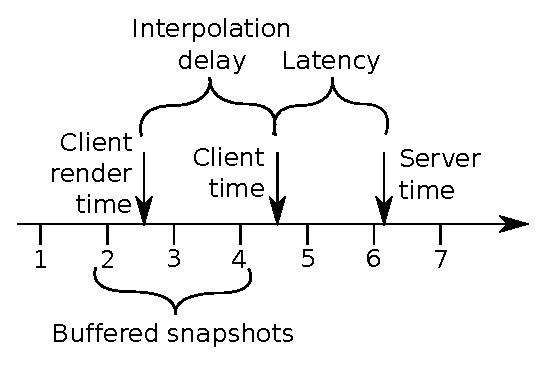
\includegraphics[width=\linewidth]{figures/interpolation_timeline.eps}
		\caption{A timeline showing delayed presentation. The client buffers updates received from the server for a short period instead of displaying them immediately. Under this scheme the client always has at least two snapshots to interpolate between, eliminating the need for prediction/dead reckoning.}
		\label{fig:interpolation_timeline}
	\end{figure}

	\section{Server-side lag compensation}

	\subsection{No compensation}

	The simplest approach to server-side lag compensation is to do nothing at all. If the clients are already predicting future world states via extrapolation, then the server doesn't need to do anything. If the clients are \emph{not} predicting future world states (for example, if they follow the buffering/interpolation approach detailed above), then a consequence of not applying server-side lag compensation is that players must lead their targets by an amount proportional to their latency and (if applicable) the interpolation period.

	\subsection{Authoritative clients}

	Another very simple approach is to make clients authoritative over their actions. For example, if the client says ``I am now at position X and I have killed player Y'', the server will just blindly accept this new information, move the player to position X, and mark player Y as dead. This only works if all clients can be trusted, which immediately rules out most real-world scenarios due to the possibility of cheating.

	\subsection{Buffering of world state}

	\cite{bernier2001latency}

	\begin{itemize}
		\item Buffer 1 sec of previous world states
		\item When a client command arrives, rewind time based on their latency and (if applicable) their interp amount, interpolating between wold states if the command occurred between ticks
		\item Execute the command in the context of this world state
		\item This can cause temporal paradoxes - players can be shot after they duck behind cover. Usually a tradeoff the developer is willing to make since it ensures responsiveness for all players
		\item If player latency varies too much (for example, if data follows many different routes), this is inaccurate. Works best if constant latency can be guaranteed
		\item Gives ``peek advantage'' when players go round corners, more pronounced if there is a large latency difference between the players in the exchange
	\end{itemize}

	\section{Network-level}

	TODO \cite{yu2008latency} \cite{yu2012latency}

	\section{Supporting technologies}

	\subsection{Clock synchronisation}

	TODO \cite{cristian1989probabilistic}

	\subsection{Delta encoding}

	No sources found yet, other than Quake 3 source code

	\section{Unified frameworks}

	TODO \cite{savery2013timelines} \cite{touch1992mirage} \cite{diot1999distributed}

	\section{Conclusions}

	TODO

	\printbibliography

\end{document}
